\documentclass[
    oneside,
    ngerman,
    footinclude=false,
    captions=tableheading,
    DIV=12
]{scrartcl}


\usepackage{UniLaTeXPackage}

\ihead{Tom Folgmann,\\David Jannack}
\chead{TUTOR\\Blattsammlung}
\ohead{\today}

\begin{document}
    \aufgabe{}
        \subaufgabe{}
            \paragraph*{Lösung mit Euler (explizit)}
                Die folgenden Graphen zeigen je die zeitliche Entwicklung von Ort, Geschwindigkeit und Energie, sowie die Ort-Geschwindigkeit-Phasenräume für verschiedene Zeitschritte.     

                \subparagraph*{Zeitschritt $0.1$}\,
                \begin{figure}[H]
                    \centering
                    \begin{subfigure}[b]{0.45\textwidth}
                        \centering
                        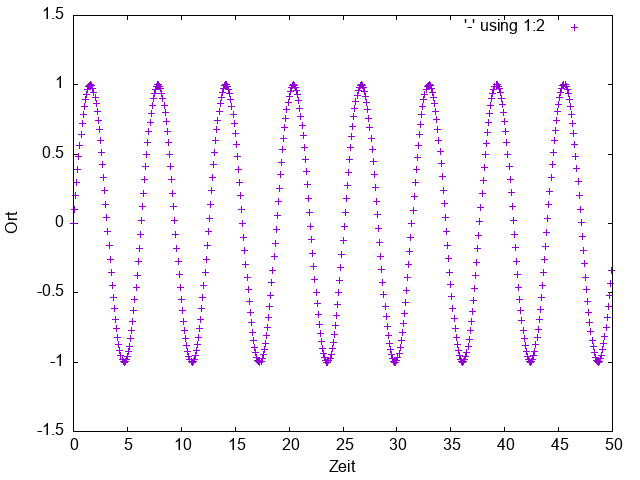
\includegraphics[width=\textwidth]{Bilddateien/expEulerA1(a)-01-0-x.png}
                        \caption{Orts-Zeit-Diagramm}
                        \label{fig:expEulerA1(a)-01-0-x}
                    \end{subfigure}
                    \hfill
                    \begin{subfigure}[b]{0.45\textwidth}
                        \centering
                        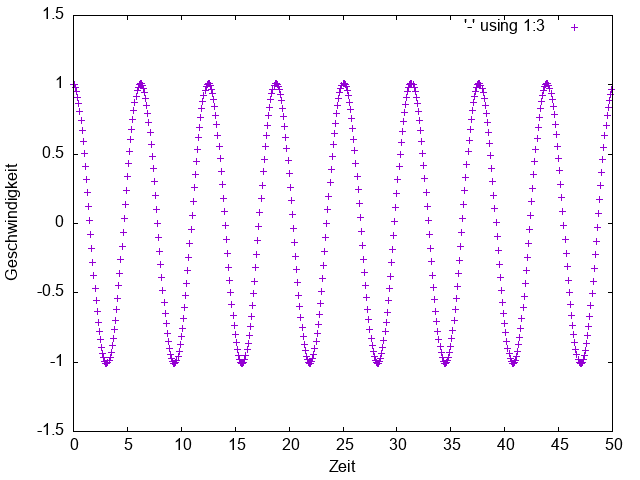
\includegraphics[width=\textwidth]{Bilddateien/expEulerA1(a)-01-0-v.png}
                        \caption{Geschwindigkeit-Zeit-Diagramm}
                        \label{fig:expEulerA1(a)-01-0-v}
                    \end{subfigure}
               \end{figure}
               Beide Diagramme zeigen eine harmonische Schwingung mit gut konstanter Amplitude, wobei beide Schwingungen phasenversetzt sind. Wir haben also eine hohe Übereinstimmung mit der Theorie. Im unteren Diagramm ist die Energie und der Phasenraum für die Schwingung gezeigt.
               
               \begin{figure}[H]
                \centering
                \begin{subfigure}[b]{0.45\textwidth}
                    \centering
                    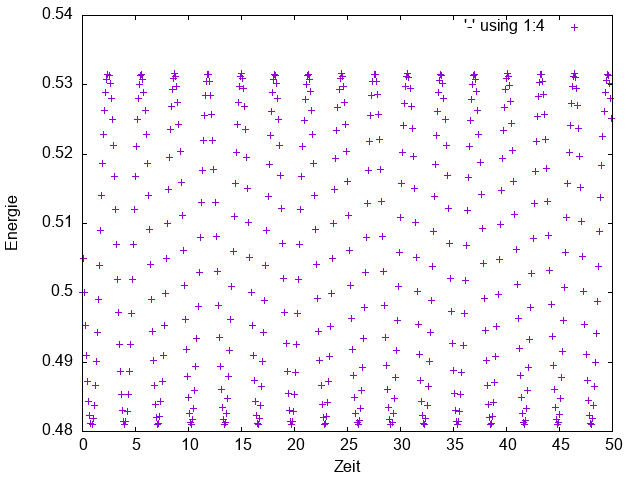
\includegraphics[width=\textwidth]{Bilddateien/expEulerA1(a)-01-E.png}
                    \caption{Energie-Zeit-Diagramm}
                    \label{fig:expEulerA1(a)-01-0-E}
                \end{subfigure}
                \hfill
                \begin{subfigure}[b]{0.45\textwidth}
                    \centering
                    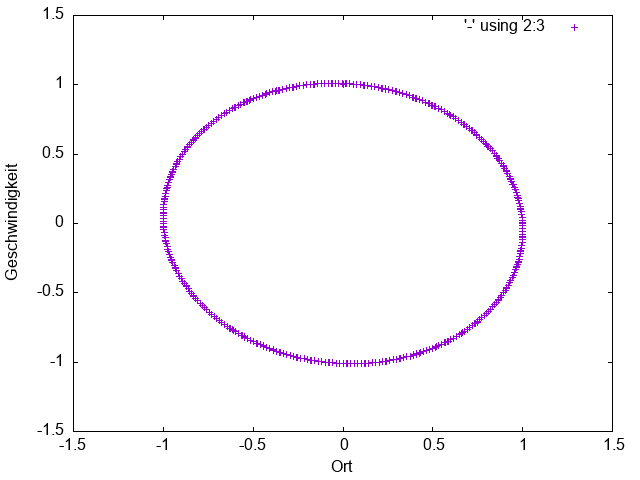
\includegraphics[width=\textwidth]{Bilddateien/expEulerA1(a)-01-0-xv.png}
                    \caption{Ort-Geschwindigkeit-Phasenraum}
                    \label{fig:expEulerA1(a)-01-0-xv}
                \end{subfigure}
                \end{figure}
                Die Energie führt bei diesem Zeitschritt noch größere Schwingungen aus, bleibt aber im Mittel konstant. Dies man auch gut daran ablesen kann, dass im Phasenraum eine zwar geschlossene, aber unsymmetrische Ellipse zu sehen ist.
                \newpage

                \subparagraph*{Zeitschritt $0.01$}\,
                \begin{figure}[H]
                    \centering
                    \begin{subfigure}[b]{0.45\textwidth}
                        \centering
                        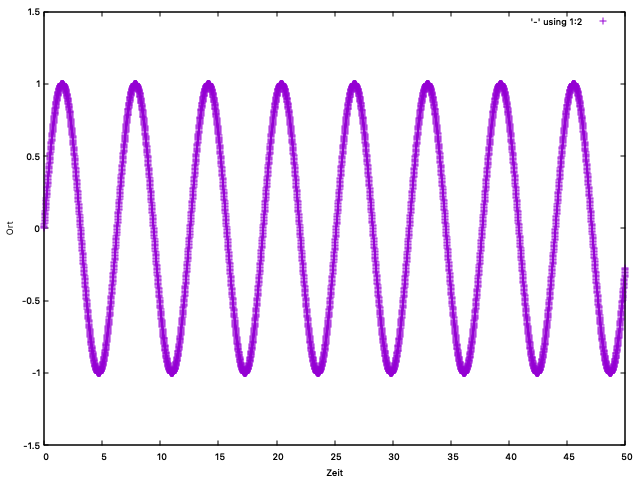
\includegraphics[width=\textwidth]{Bilddateien/expEulerA1(a)-001h-x.png}
                        \caption{Orts-Zeit-Diagramm}
                        \label{fig:expEulerA1(a)-001-0-x}
                    \end{subfigure}
                    \hfill
                    \begin{subfigure}[b]{0.45\textwidth}
                        \centering
                        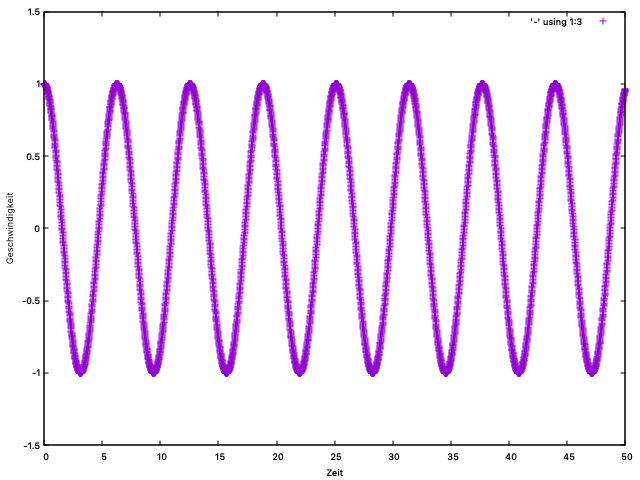
\includegraphics[width=\textwidth]{Bilddateien/expEulerA1(a)-001h-v.png}
                        \caption{Geschwindigkeit-Zeit-Diagramm}
                        \label{fig:expEulerA1(a)-001-0-v}
                    \end{subfigure}
                \end{figure}
                
                \begin{figure}[H]
                \centering
                \begin{subfigure}[b]{0.45\textwidth}
                    \centering
                    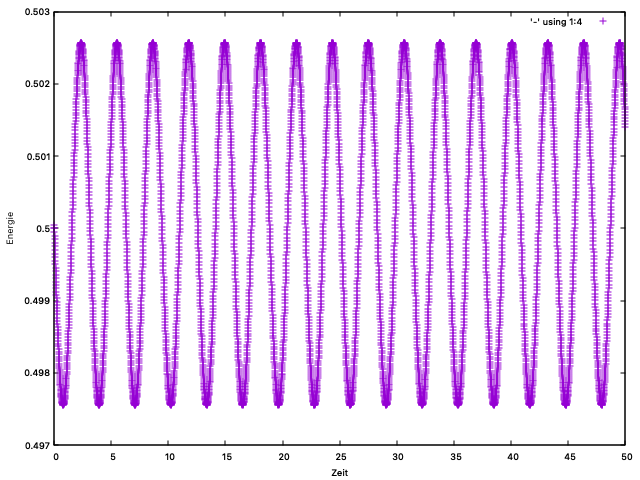
\includegraphics[width=\textwidth]{Bilddateien/expEulerA1(a)-001h-E.png}
                    \caption{Energie-Zeit-Diagramm}
                    \label{fig:expEulerA1(a)-001-0-E}
                \end{subfigure}
                \end{figure}
                Auch hier schwingt die Energie, aber mit kleinerer Ampltiude.
                \newpage

                \subparagraph*{Zeitschritt $0.001$}\,
                \begin{figure}[H]
                    \centering
                    \begin{subfigure}[b]{0.45\textwidth}
                        \centering
                        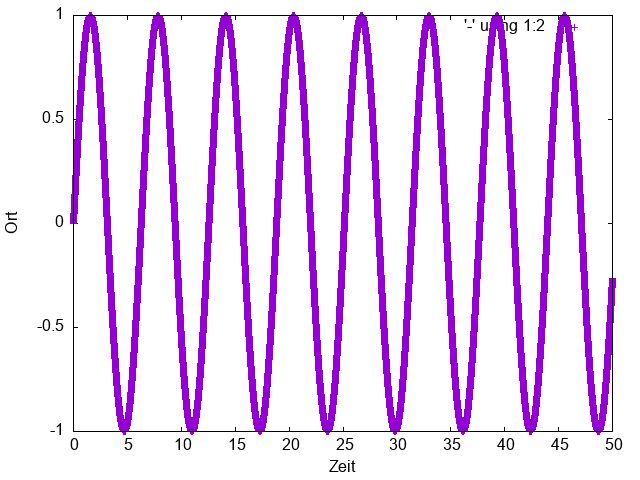
\includegraphics[width=\textwidth]{Bilddateien/expEulerA1(a)-0001-0-x.png}
                        \caption{Orts-Zeit-Diagramm}
                        \label{fig:expEulerA1(a)-0001-0-x}
                    \end{subfigure}
                    \hfill
                    \begin{subfigure}[b]{0.45\textwidth}
                        \centering
                        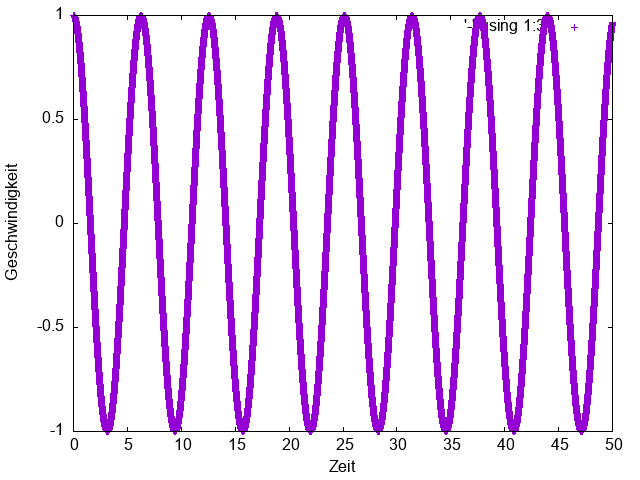
\includegraphics[width=\textwidth]{Bilddateien/expEulerA1(a)-0001-0-v.png}
                        \caption{Geschwindigkeit-Zeit-Diagramm}
                        \label{fig:expEulerA1(a)-0001-0-v}
                    \end{subfigure}
                \end{figure}
                
                \begin{figure}[H]
                \centering
                \begin{subfigure}[b]{0.45\textwidth}
                    \centering
                    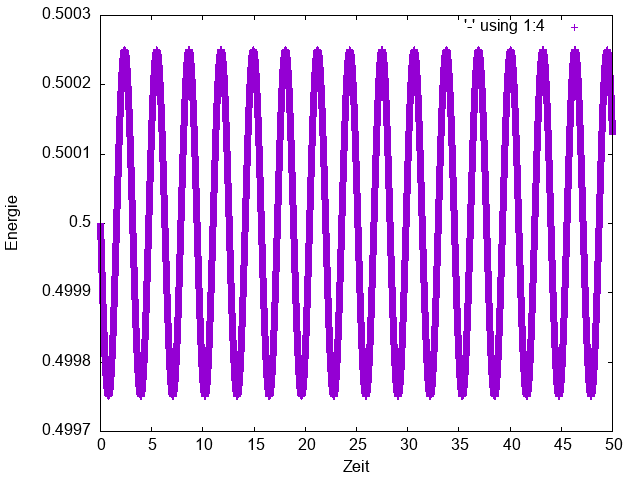
\includegraphics[width=\textwidth]{Bilddateien/expEulerA1(a)-0001-E.png}
                    \caption{Orts-Zeit-Diagramm}
                    \label{fig:expEulerA1(a)-0001-0-E}
                \end{subfigure}
                \hfill
                \begin{subfigure}[b]{0.45\textwidth}
                    \centering
                    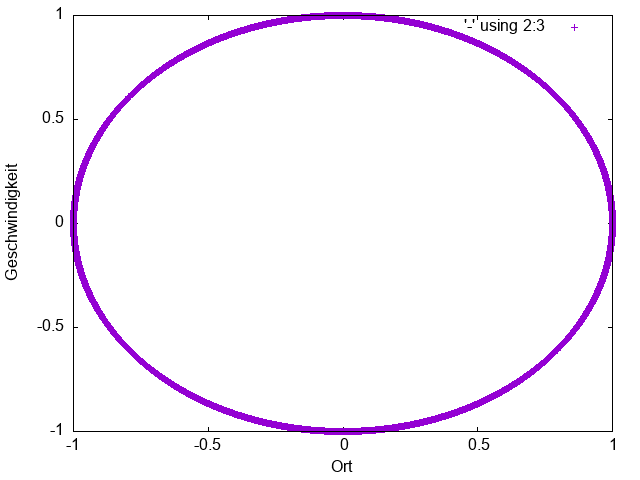
\includegraphics[width=\textwidth]{Bilddateien/expEulerA1(a)-0001-0-xv.png}
                    \caption{Energie-Geschwindigkeit-Phasenraum}
                    \label{fig:expEulerA1(a)-0001-0-xv}
                \end{subfigure}
            \end{figure}
            Die Energie variiert hier nur noch sehr wenig, was sich in einer recht idealen Ellipse im Phasenraum äußert.
            \newpage

        \paragraph*{Lösung mit leap-frog}
            \subparagraph*{Zeitschritt $0.1$}\,
            \begin{figure}[H]
                \centering
                \begin{subfigure}[b]{0.45\textwidth}
                    \centering
                    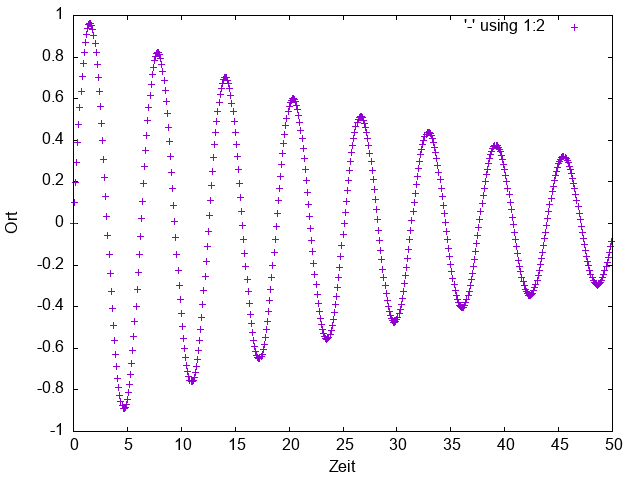
\includegraphics[width=\textwidth]{Bilddateien/LLA1(a)-01-0-x.png}
                    \caption{Orts-Zeit-Diagramm}
                    \label{fig:LLA1(a)-01-0-x}
                \end{subfigure}
                \hfill
                \begin{subfigure}[b]{0.45\textwidth}
                    \centering
                    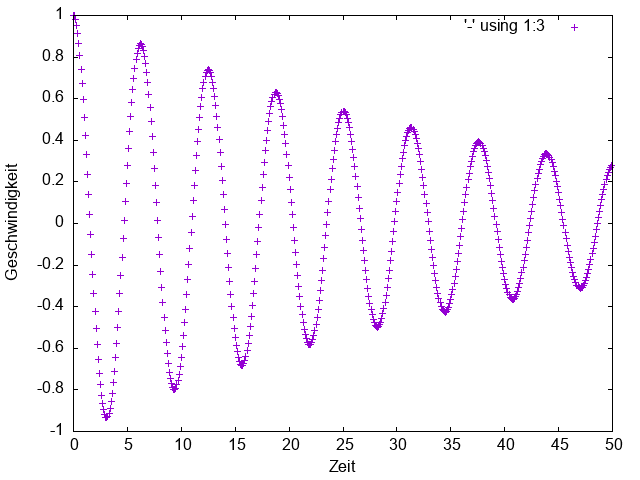
\includegraphics[width=\textwidth]{Bilddateien/LLA1(a)-01-0-v.png}
                    \caption{Geschwindigkeit-Zeit-Diagramm}
                    \label{fig:LLA1(a)-01-0-v}
                \end{subfigure}
            \end{figure}
            In beiden Diagrammen lässt sich eine Dämpfung der Schwingung erkennen, obwohl ein Dämpfungskoeffizient von $\gamma=0$ vorliegt. Für diesen Zeitrschritt ist das leap-frog-Verfahren also noch dem Eulerverfahren unterlegen.
        
            \begin{figure}[H]
            \centering
            \begin{subfigure}[b]{0.45\textwidth}
                \centering
                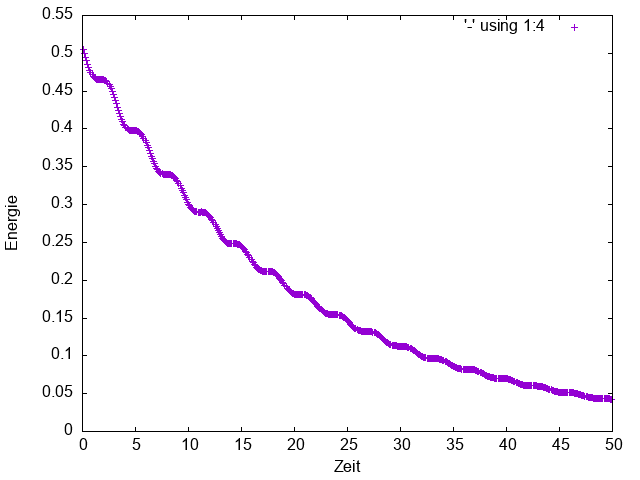
\includegraphics[width=\textwidth]{Bilddateien/LLA1(a)-01-E.png}
                \caption{Energie-Zeit-Diagramm}
                \label{fig:LLA1(a)-01-0-E}
            \end{subfigure}
            \hfill
            \begin{subfigure}[b]{0.45\textwidth}
                \centering
                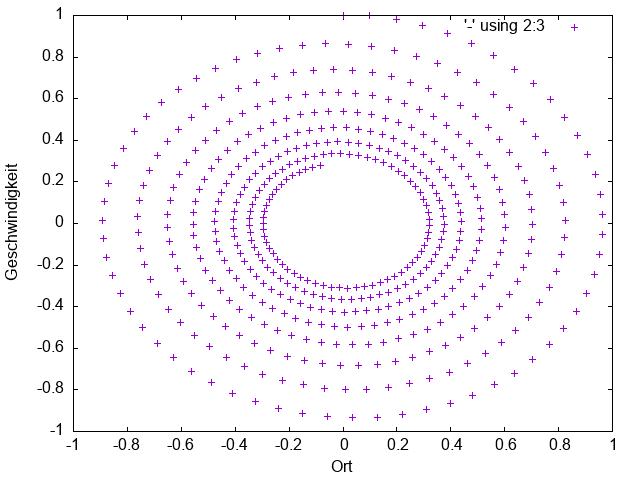
\includegraphics[width=\textwidth]{Bilddateien/LLA1(a)-01-0-xv.png}
                \caption{Ort-Geschwindigkeit-Phasenraum}
                \label{fig:LLA1(a)-01-0-xv}
            \end{subfigure}
            \end{figure}
            Wie aufgrund der Dämpfung des Schwingungen zu erwarten ist, fällt die Enerige mit der Zeit (hat aber periodische kleine lokale Maxima). Im Phasendiagramm äußert sich das in Form einer Spirale.
            \newpage

            \subparagraph*{Zeitschritt $0.01$}\,
            \begin{figure}[H]
                \centering
                \begin{subfigure}[b]{0.45\textwidth}
                    \centering
                    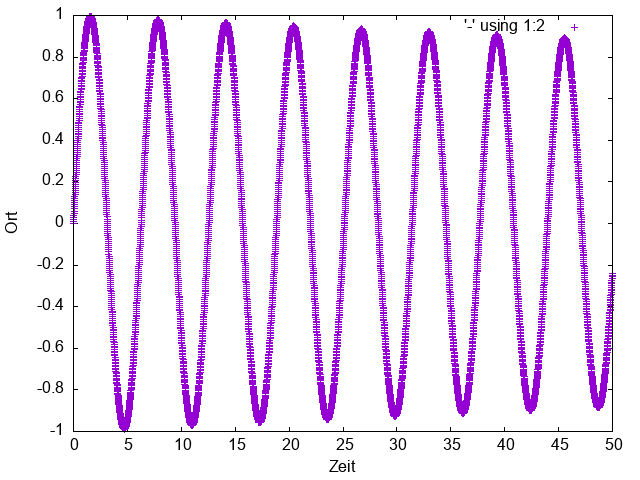
\includegraphics[width=\textwidth]{Bilddateien/LLA1(a)-001-0-x.png}
                    \caption{Orts-Zeit-Diagramm}
                    \label{fig:LLA1(a)-001-0-x}
                \end{subfigure}
                \hfill
                \begin{subfigure}[b]{0.45\textwidth}
                    \centering
                    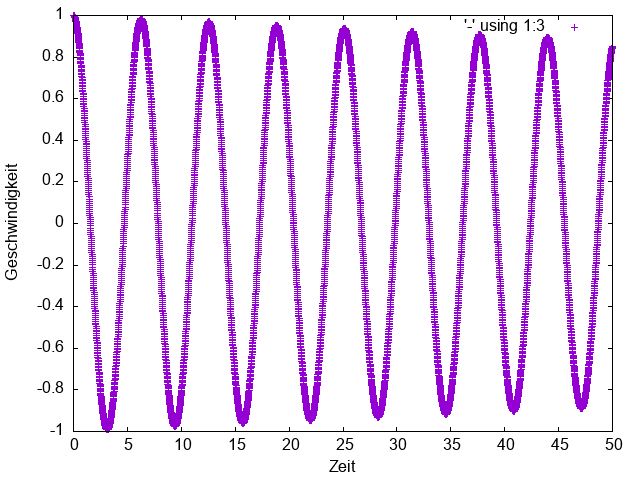
\includegraphics[width=\textwidth]{Bilddateien/LLA1(a)-001-0-v.png}
                    \caption{Geschwindigkeit-Zeit-Diagramm}
                    \label{fig:LLA1(a)-001-0-v}
                \end{subfigure}
            \end{figure}
            Mit kleineren Zeitschritte ist auch die Dämpfung der Schwingung kleiner, es handelt sich also tatsächlich um einen numerischen Fehler.
            
            \begin{figure}[H]
            \centering
            \begin{subfigure}[b]{0.45\textwidth}
                \centering
                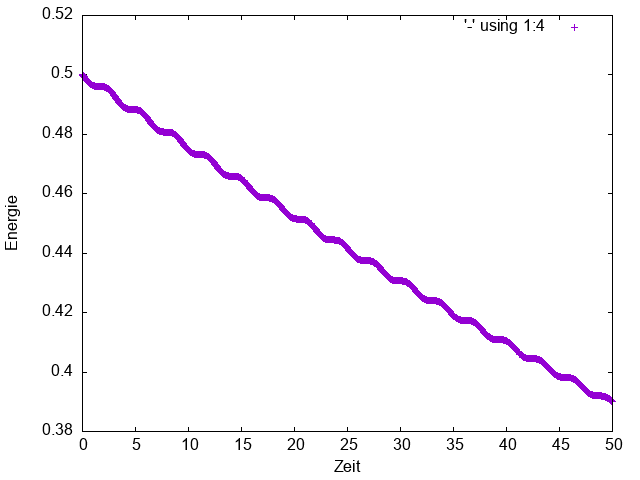
\includegraphics[width=\textwidth]{Bilddateien/LLA1(a)-001-E.png}
                \caption{Energie-Zeit-Diagramm}
                \label{fig:LLA1(a)-001-0-E}
            \end{subfigure}
            \hfill
            \begin{subfigure}[b]{0.45\textwidth}
                \centering
                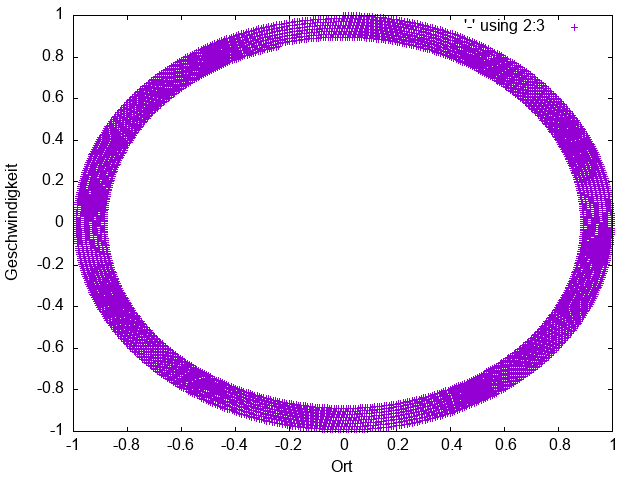
\includegraphics[width=\textwidth]{Bilddateien/LLA1(a)-001-0-xv.png}
                \caption{Ort-Geschwindigkeit-Phasenraum}
                \label{fig:LLA1(a)-001-0-xv}
            \end{subfigure}
            \end{figure}
            Im Phasendiagramm äußert sich die kleinere Energiedissizipation dadurch, dass die Spirale sehr viel länger braucht, um abzufallen.
            \newpage

            \subparagraph*{Zeitschritt $0.001$}\,
            \begin{figure}[H]
                \centering
                \begin{subfigure}[b]{0.45\textwidth}
                    \centering
                    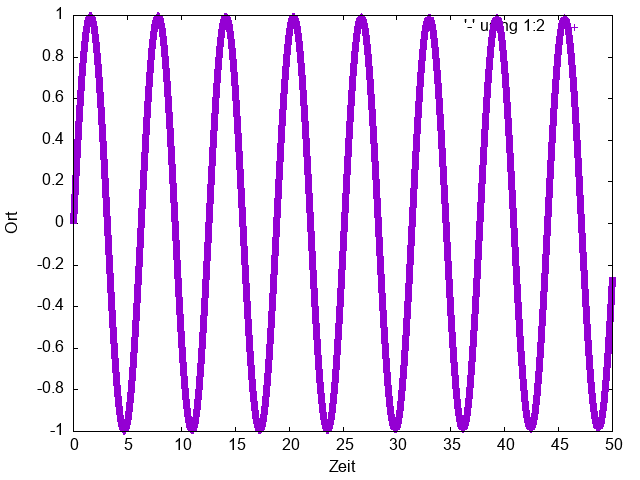
\includegraphics[width=\textwidth]{Bilddateien/LLA1(a)-0001-0-x.png}
                    \caption{Orts-Zeit-Diagramm}
                    \label{fig:LLA1(a)-0001-0-x}
                \end{subfigure}
                \hfill
                \begin{subfigure}[b]{0.45\textwidth}
                    \centering
                    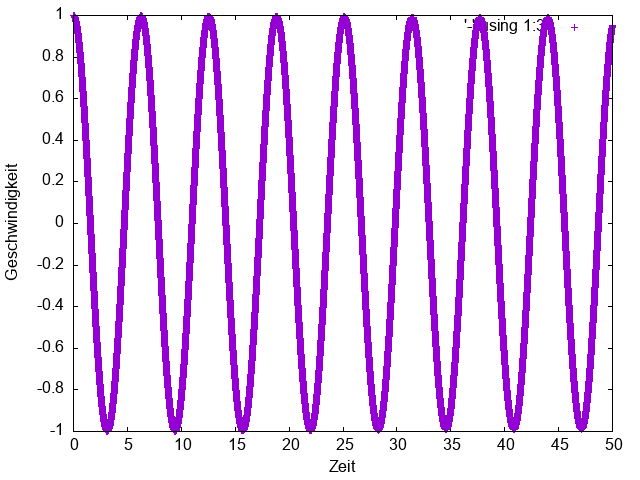
\includegraphics[width=\textwidth]{Bilddateien/LLA1(a)-0001-0-v.png}
                    \caption{Geschwindigkeit-Zeit-Diagramm}
                    \label{fig:LLA1(a)-0001-0-v}
                \end{subfigure}
            \end{figure}
            Für $h=0.001$ ist die Amplitude nun nahezu konstant.
            
            \begin{figure}[H]
            \centering
            \begin{subfigure}[b]{0.45\textwidth}
                \centering
                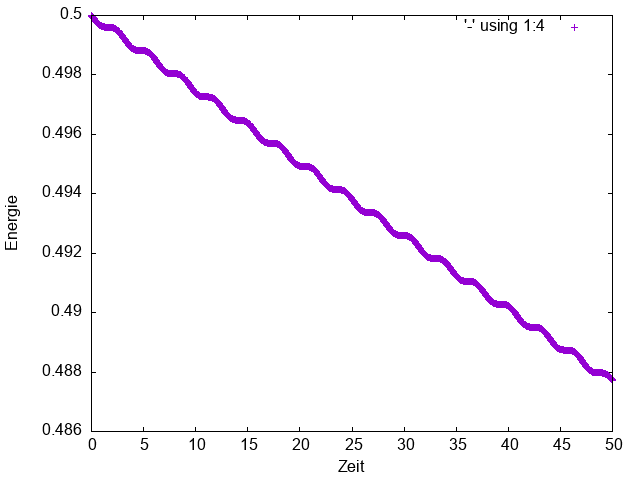
\includegraphics[width=\textwidth]{Bilddateien/LLA1(a)-0001-E.png}
                \caption{Energie-Zeit-Diagramm}
                \label{fig:LLA1(a)-0001-0-E}
            \end{subfigure}
            \hfill
            \begin{subfigure}[b]{0.45\textwidth}
                \centering
                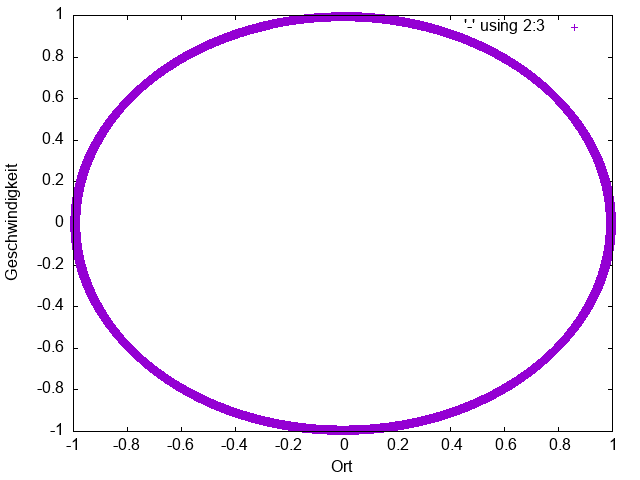
\includegraphics[width=\textwidth]{Bilddateien/LLA1(a)-0001-0-xv.png}
                \caption{Ort-Geschwindigkeit-Phasenraum}
                \label{fig:LLA1(a)-0001-0-xv}
            \end{subfigure}
            \end{figure}
            Auch die Energie hat eine sehr viel kleinere Steigung und die Spirale ähnelt sehr einer Ellipse. Allerdings deutet die im Vergleich zum expliziten Eulerverfahren dickeren "Ränder" an, dass dieses immernoch akkurater ist hier.
            \newpage

        \paragraph*{Lösung mit Runge-Kutta (2. Ordnung)}
            \subparagraph*{Zeitschritt $0.1$}\,
            \begin{figure}[H]
                \centering
                \begin{subfigure}[b]{0.45\textwidth}
                    \centering
                    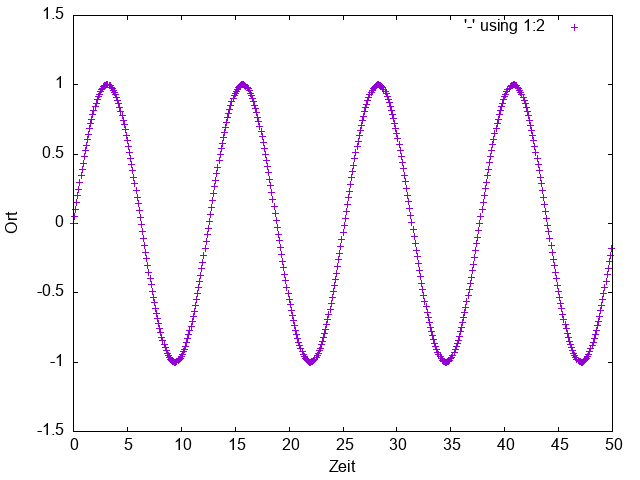
\includegraphics[width=\textwidth]{Bilddateien/RK2A1(a)-01-0-x.png}
                    \caption{Orts-Zeit-Diagramm}
                    \label{fig:RK2A1(a)-01-0-x}
                \end{subfigure}
                \hfill
                \begin{subfigure}[b]{0.45\textwidth}
                    \centering
                    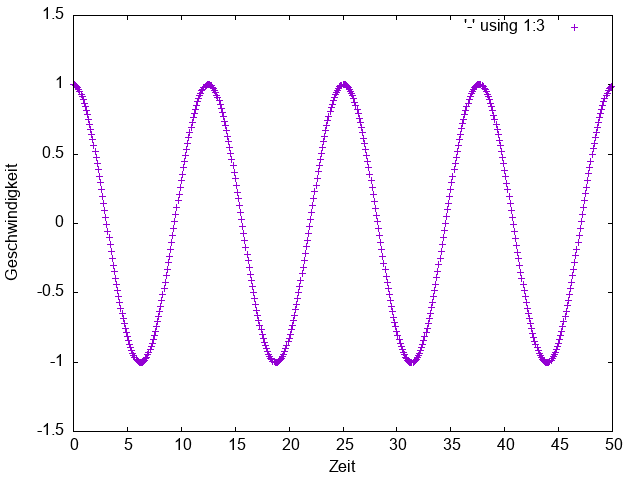
\includegraphics[width=\textwidth]{Bilddateien/RK2A1(a)-01-0-v.png}
                    \caption{Geschwindigkeit-Zeit-Diagramm}
                    \label{fig:RK2A1(a)-01-0-v}
                \end{subfigure}
            \end{figure}
            Für das Runge-Kutta Verfahren 2. Ordnung zeigt sich bereits für kleine Zeitschritte ein stabiles Verhalten bei der Amplitude.
        
            \begin{figure}[H]
            \centering
            \begin{subfigure}[b]{0.45\textwidth}
                \centering
                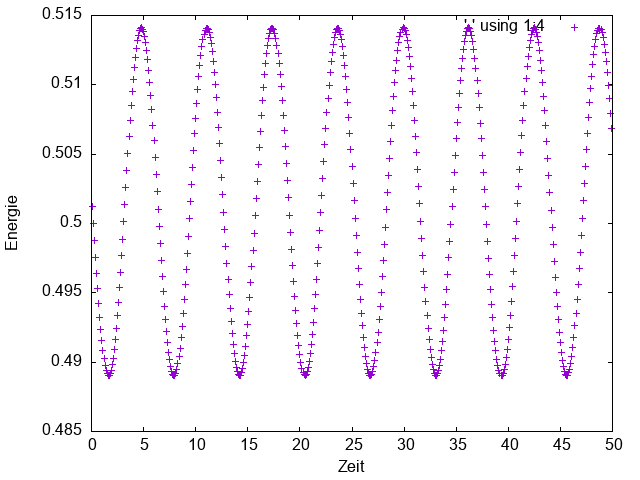
\includegraphics[width=\textwidth]{Bilddateien/RK2A1(a)-01-E.png}
                \caption{Energie-Zeit-Diagramm}
                \label{fig:RK2A1(a)-01-0-E}
            \end{subfigure}
            \hfill
            \begin{subfigure}[b]{0.45\textwidth}
                \centering
                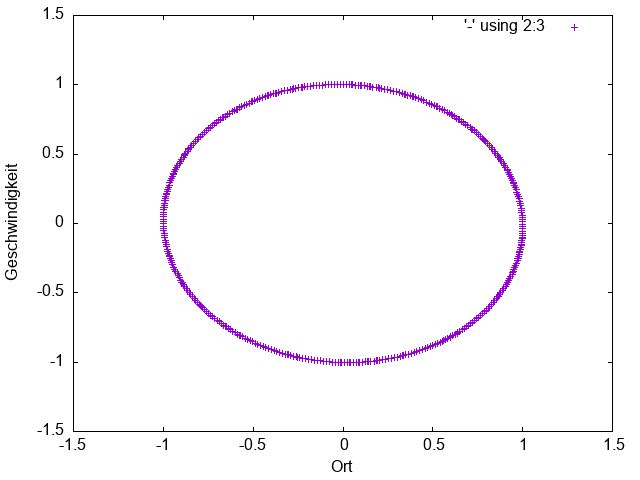
\includegraphics[width=\textwidth]{Bilddateien/RK2A1(a)-01-0-xv.png}
                \caption{Ort-Geschwindigkeit-Phasenraum}
                \label{fig:RK2A1(a)-01-0-xv}
            \end{subfigure}
            \end{figure}
            Die Energie oszilliert auch hier noch, aber weniger als beim Euler-Verfahren.
            \newpage

            \subparagraph*{Zeitschritt $0.001$}\,
            \begin{figure}[H]
                \centering
                \begin{subfigure}[b]{0.45\textwidth}
                    \centering
                    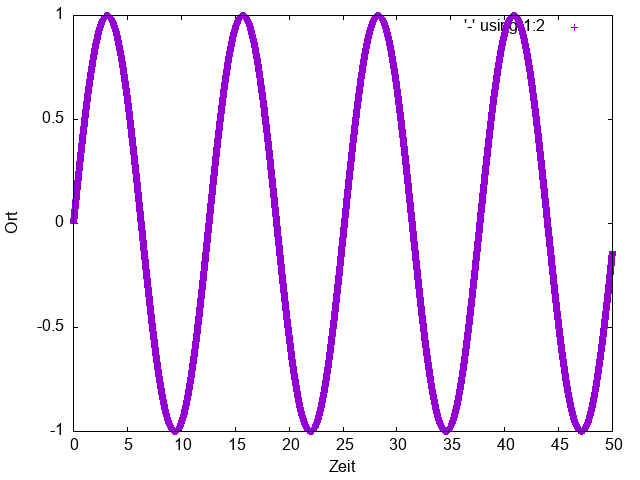
\includegraphics[width=\textwidth]{Bilddateien/RK2A1(a)-0001-0-x.png}
                    \caption{Orts-Zeit-Diagramm}
                    \label{fig:RK2A1(a)-0001-0-x}
                \end{subfigure}
                \hfill
                \begin{subfigure}[b]{0.45\textwidth}
                    \centering
                    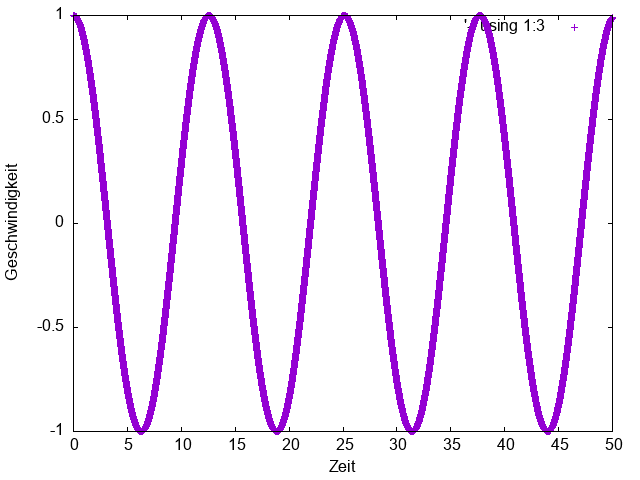
\includegraphics[width=\textwidth]{Bilddateien/RK2A1(a)-0001-0-v.png}
                    \caption{Geschwindigkeit-Zeit-Diagramm}
                    \label{fig:RK2A1(a)-0001-0-v}
                \end{subfigure}
            \end{figure}
        
            \begin{figure}[H]
            \centering
            \begin{subfigure}[b]{0.45\textwidth}
                \centering
                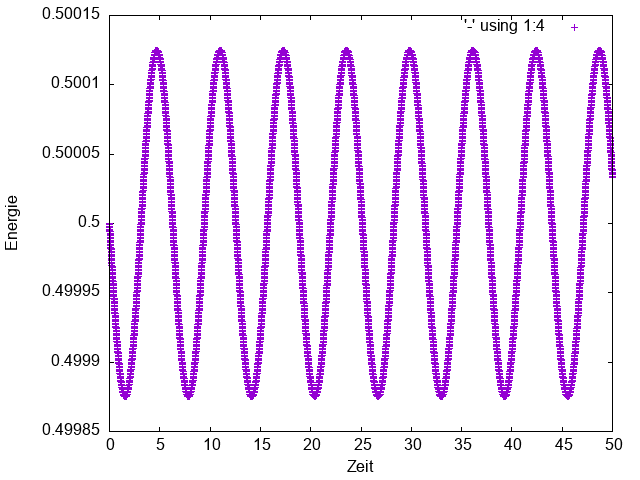
\includegraphics[width=\textwidth]{Bilddateien/RK2A1(a)-0001-E.png}
                \caption{Energie-Zeit-Diagramm}
                \label{fig:RK2A1(a)-0001-0-E}
            \end{subfigure}
            \hfill
            \begin{subfigure}[b]{0.45\textwidth}
                \centering
                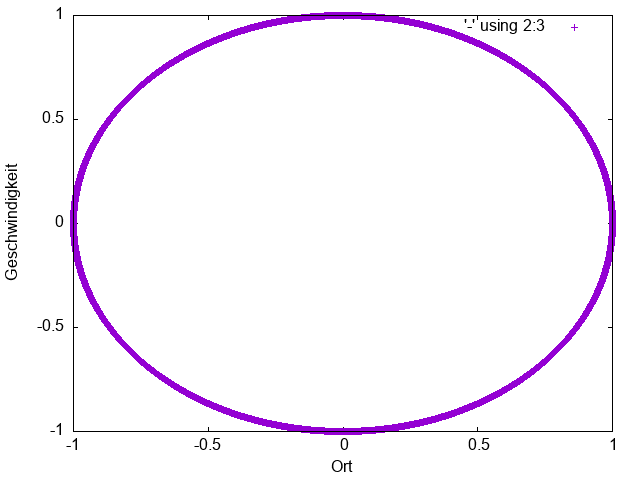
\includegraphics[width=\textwidth]{Bilddateien/RK2A1(a)-0001-0-xv.png}
                \caption{Ort-Geschwindigkeit-Phasenraum}
                \label{fig:RK2A1(a)-0001-0-xv}
            \end{subfigure}
            \end{figure}
            Bei sehr kleinen Zeitschritten von $h=0.001$ ist die Energie bis zur dritten Nachkommastelle konstant und die Ellipse im Phasenraum dementsprechend ideal. Somit ist das Runge-Kutta-Verfahren wie zu erwarten am genauesten.
            \newpage

        \subaufgabe{}
            Wir betrachten nun die numerische Lösung des gedämpften Oszillators für verschiedene Dämpfungskoeffizienten $\gamma$, wobei wir das Verlet-Verfahren nutzen. $\gamma$ ist über $F_{Reibung}(t)=-\gamma\cdot \dot x(t)$ definiert. Als Zeitschrittweite nehmen wir $h=0.01$

            \paragraph{Schwingfall}
                \subparagraph{Dämpfung $\gamma=0.3$}\,
                \begin{figure}[H]
                    \centering
                    \begin{subfigure}[b]{0.45\textwidth}
                        \centering
                        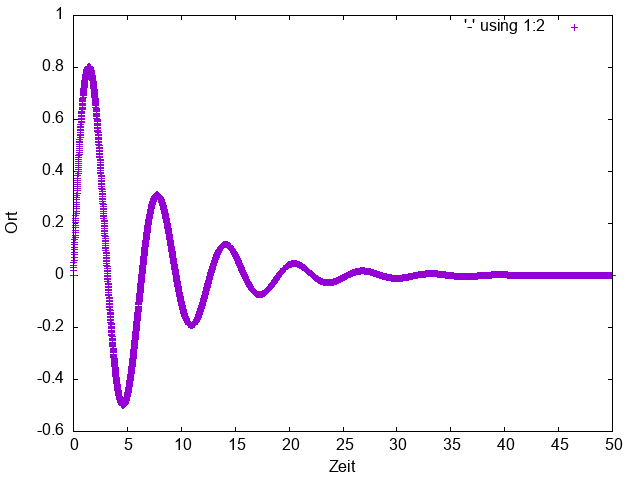
\includegraphics[width=\textwidth]{Bilddateien/VVA1(b)-001-0.3-x.png}
                        \caption{Ort-Zeit-Diagramm}
                        \label{fig:VVA1(a)-001-0.3-x}
                    \end{subfigure}
                    \hfill
                    \begin{subfigure}[b]{0.45\textwidth}
                        \centering
                        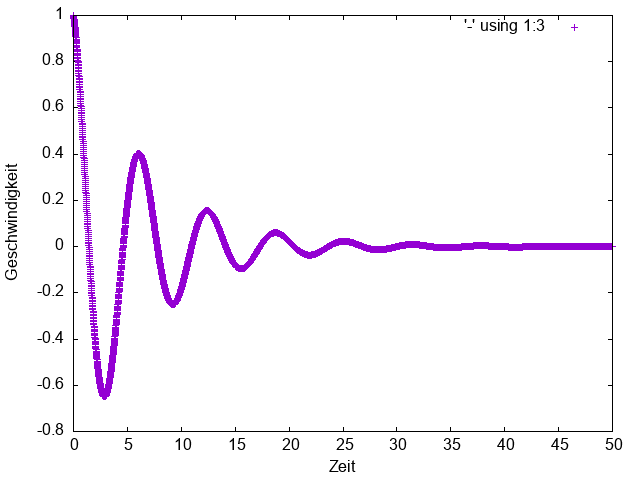
\includegraphics[width=\textwidth]{Bilddateien/VVA1(b)-001-0.3-v.png}
                        \caption{Geschwindigkeit-Zeit-Diagramm}
                        \label{fig:VVA1(a)-001-0.3-v}
                    \end{subfigure}
                    \hfill
                    \begin{subfigure}[b]{0.45\textwidth}
                        \centering
                        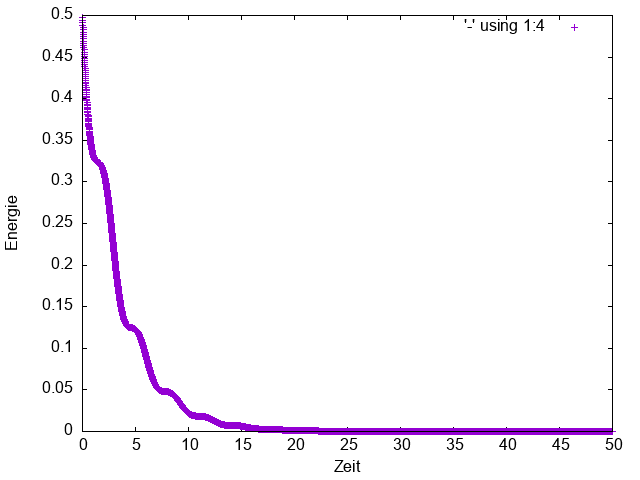
\includegraphics[width=\textwidth]{Bilddateien/VVA1(b)-001-0.3-E.png}
                        \caption{Energie-Zeit-Phasenraum}
                        \label{fig:VVA1(a)-001-0.3-E}
                    \end{subfigure}
                    \begin{subfigure}[b]{0.45\textwidth}
                        \centering
                        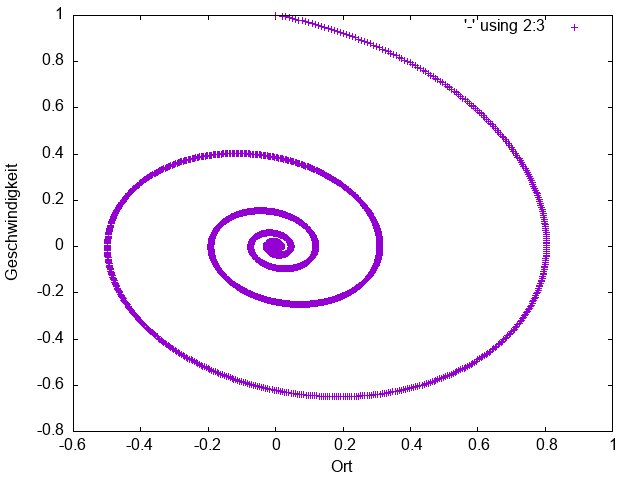
\includegraphics[width=\textwidth]{Bilddateien/VVA1(b)-001-0.3-xv.png}
                        \caption{Ort-Geschwindigkeit-Phasenraum}
                        \label{fig:VVA1(a)-001-0.3-xv}
                    \end{subfigure}
                \end{figure}
                Für leichte Dämpfung lässt sich der Schwingfall beoachten, der eine harmonische Schwingungen mit exponentiell abfallender Amplitude darstellt. Im Phasendiagramm resultiert dies in einer nicht-symmetrischen Spirale.
                \newpage

                \subparagraph{Dämpfung $\gamma=0.7$}\,
                \begin{figure}[H]
                    \centering
                    \begin{subfigure}[b]{0.45\textwidth}
                        \centering
                        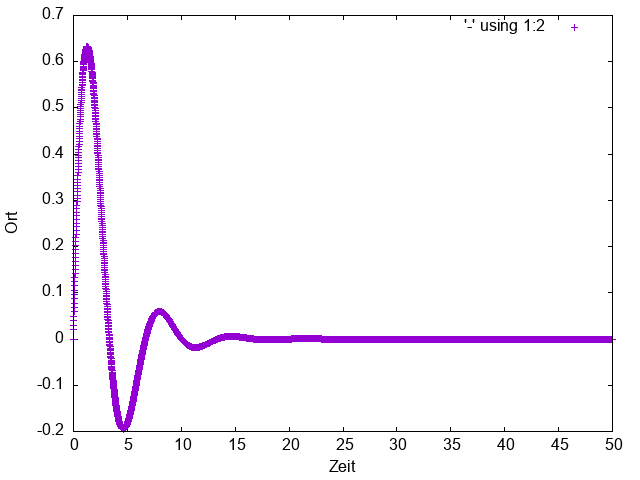
\includegraphics[width=\textwidth]{Bilddateien/VVA1(b)-001-0.7-x.png}
                        \caption{Ort-Zeit-Diagramm}
                        \label{fig:VVA1(a)-001-0.7-x}
                    \end{subfigure}
                    \hfill
                    \begin{subfigure}[b]{0.45\textwidth}
                        \centering
                        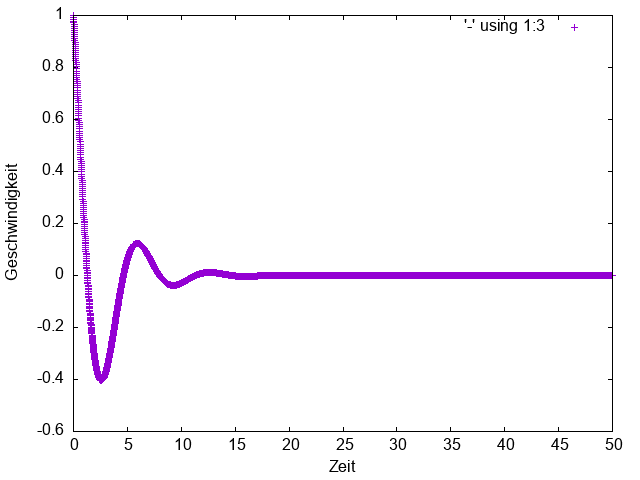
\includegraphics[width=\textwidth]{Bilddateien/VVA1(b)-001-0.7-v.png}
                        \caption{Geschwindigkeit-Zeit-Diagramm}
                        \label{fig:VVA1(a)-001-0.7-v}
                    \end{subfigure}
                    \begin{subfigure}[b]{0.45\textwidth}
                        \centering
                        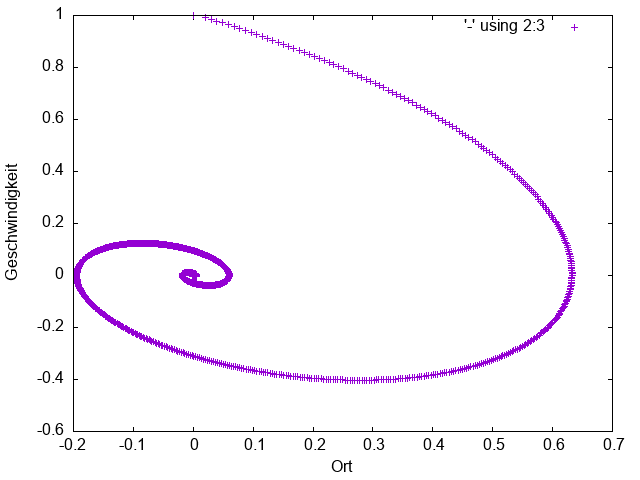
\includegraphics[width=\textwidth]{Bilddateien/VVA1(b)-001-0.7-xv.png}
                        \caption{Ort-Geschwindigkeit-Phasenraum}
                        \label{fig:VVA1(a)-001-0.7-xv}
                    \end{subfigure}
                \end{figure}
                Auch für $\gamma=0.7$ ist noch der Schwingfall vorhanden, allerdings werden deutlich weniger Schwingungen mit sichtbarer Amplitde ausgeführt; die Spirale im Phasenraumdiagramm konvergiert schneller gegen den Ursprung.
                \newpage
            
            \paragraph{Aperiodischer Grenzfall}
                \subparagraph{Dämpfung $\gamma=1.5$}\,
                \begin{figure}[H]
                    \centering
                    \begin{subfigure}[b]{0.45\textwidth}
                        \centering
                        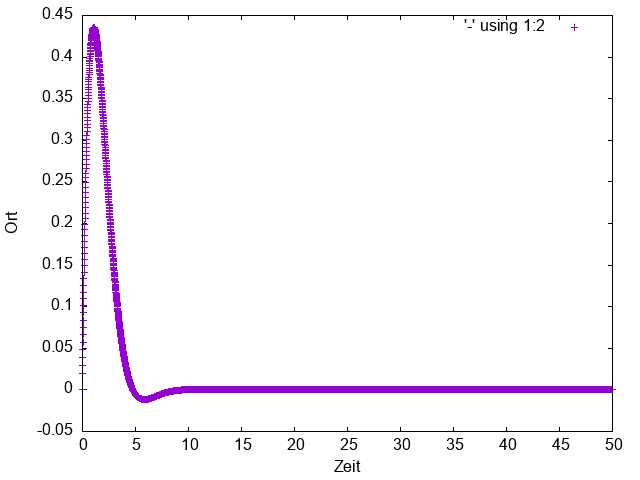
\includegraphics[width=\textwidth]{Bilddateien/VVA1(b)-001-1.5-x.png}
                        \caption{Ort-Zeit-Diagramm}
                        \label{fig:VVA1(a)-001-1.5-x}
                    \end{subfigure}
                    \hfill
                    \begin{subfigure}[b]{0.45\textwidth}
                        \centering
                        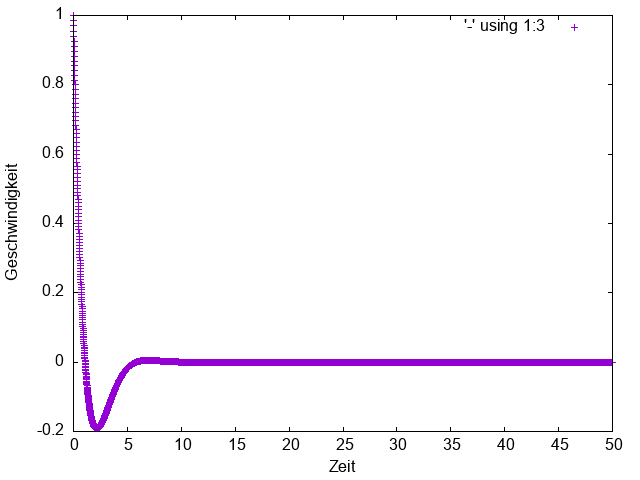
\includegraphics[width=\textwidth]{Bilddateien/VVA1(b)-001-1.5-v.png}
                        \caption{Geschwindigkeit-Zeit-Diagramm}
                        \label{fig:VVA1(a)-001-1.5-v}
                    \end{subfigure}
                    \begin{subfigure}[b]{0.45\textwidth}
                        \centering
                        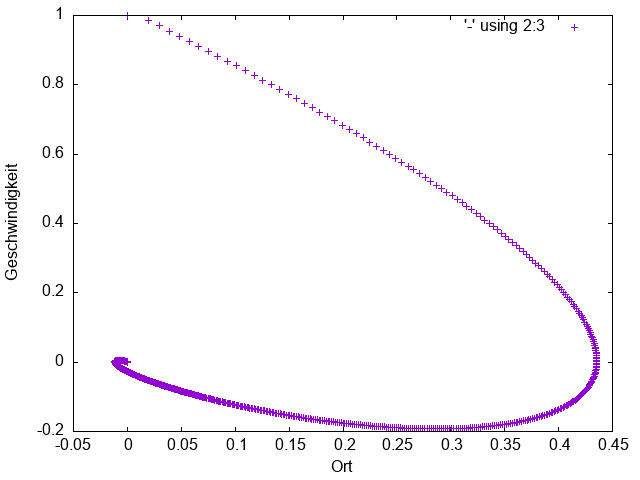
\includegraphics[width=\textwidth]{Bilddateien/VVA1(b)-001-1.5-xv.png}
                        \caption{Ort-Geschwindigkeit-Phasenraum}
                        \label{fig:VVA1(a)-001-1.5-xv}
                    \end{subfigure}
                \end{figure}
                Im Aperiodischen Grenzfall kann der Oszillator nach Theorie höchstens noch einen Nulldurchlauf haben. Da dies hier vorkommt, ist eben dieser Fall zu vermuten. Das Phasendiagramm zeigt weiter eine Spirale, die nocht stärker verzerrt ist und gegen den Ursprung schneller konvergiert als zuvor.
                \newpage

            \paragraph{Kriechfall}
                \subparagraph{Dämpfung $\gamma=3$}\,
                \begin{figure}[H]
                    \centering
                    \begin{subfigure}[b]{0.45\textwidth}
                        \centering
                        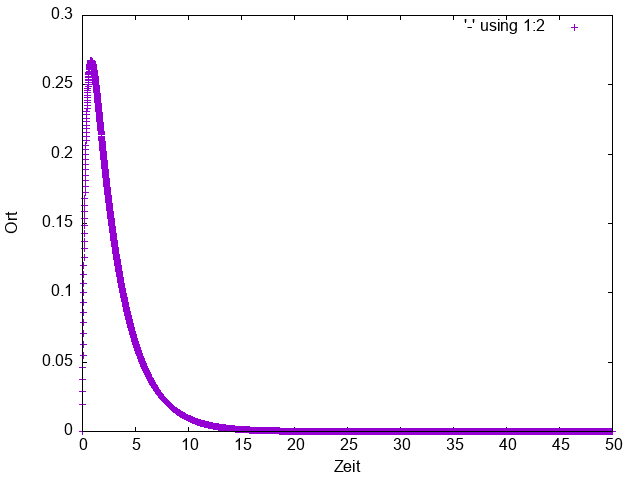
\includegraphics[width=\textwidth]{Bilddateien/VVA1(b)-001-3-x.png}
                        \caption{Ort-Zeit-Diagramm}
                        \label{fig:VVA1(a)-001-3-x}
                    \end{subfigure}
                    \hfill
                    \begin{subfigure}[b]{0.45\textwidth}
                        \centering
                        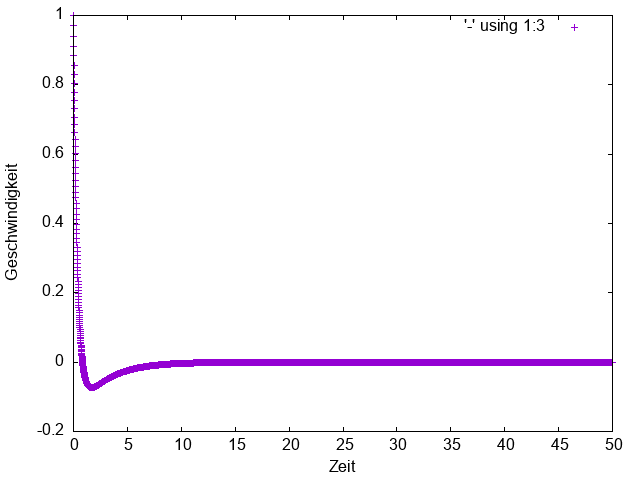
\includegraphics[width=\textwidth]{Bilddateien/VVA1(b)-001-3-v.png}
                        \caption{Geschwindigkeit-Zeit-Diagramm}
                        \label{fig:VVA1(a)-001-3-v}
                    \end{subfigure}
                    \begin{subfigure}[b]{0.45\textwidth}
                        \centering
                        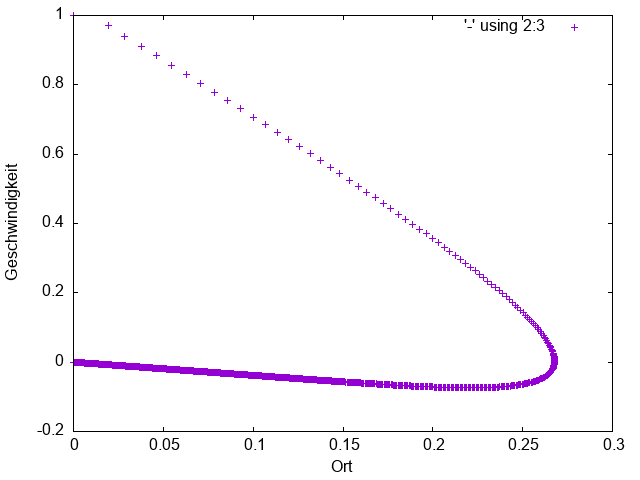
\includegraphics[width=\textwidth]{Bilddateien/VVA1(b)-001-3-xv.png}
                        \caption{Ort-Geschwindigkeit-Phasenraum}
                        \label{fig:VVA1(a)-001-3-xv}
                    \end{subfigure}
                \end{figure}
               Für $\gamma=3$ geht die Auslenkung wieder langsamer gegen Null und im Phasendiagramm ist die Spirale fast nicht mehr zu erkennen. Dies liegt vermutlich daran, dass die Geschwindigkeit kaum variiert für kleine Zeiten und so die Phasenkurve $x(v)$ fast denselben Weg wieder beschreitet.
               \newpage

               \subparagraph{Dämpfung $\gamma=10$}\,
               \begin{figure}[H]
                   \centering
                   \begin{subfigure}[b]{0.45\textwidth}
                       \centering
                       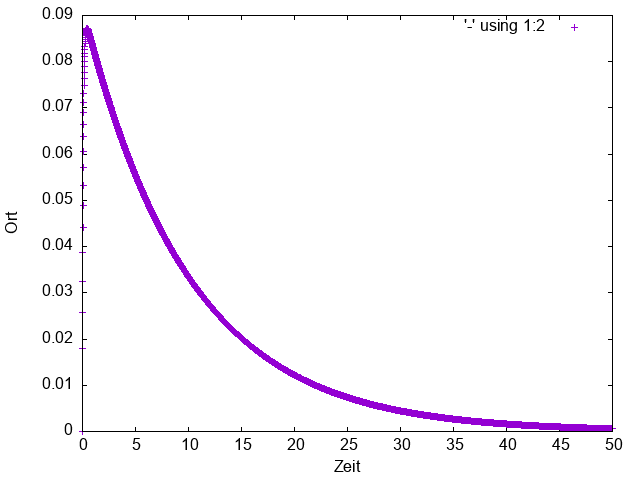
\includegraphics[width=\textwidth]{Bilddateien/VVA1(b)-001-10-x.png}
                       \caption{Ort-Zeit-Diagramm}
                       \label{fig:VVA1(a)-001-10-x}
                   \end{subfigure}
                   \hfill
                   \begin{subfigure}[b]{0.45\textwidth}
                       \centering
                       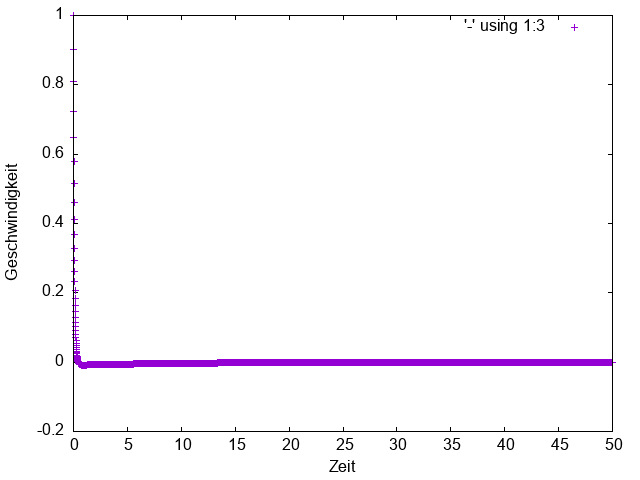
\includegraphics[width=\textwidth]{Bilddateien/VVA1(b)-001-10-v.png}
                       \caption{Geschwindigkeit-Zeit-Diagramm}
                       \label{fig:VVA1(a)-001-10-v}
                   \end{subfigure}
                   \begin{subfigure}[b]{0.45\textwidth}
                       \centering
                       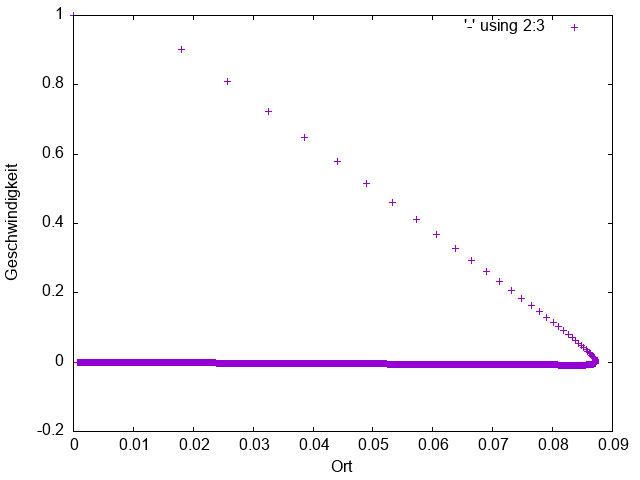
\includegraphics[width=\textwidth]{Bilddateien/VVA1(b)-001-10-xv.png}
                       \caption{Ort-Geschwindigkeit-Phasenraum}
                       \label{fig:VVA1(a)-001-10-xv}
                   \end{subfigure}
                \end{figure}
                Für $\gamma=10$ ist der Kriechfall noch deutlicher zu erkennen.

        \subaufgabe{}

        \subaufgabe{}
            

    \newpage
    \subsection*{Hauptcode}
        \lstinputlisting[language=C++]{../src/main.cpp}

    \subsection*{Headerdateien}
        \subsubsection*{Einschrittverfahren}
            \lstinputlisting[language=C++]{../src/header/Einschritt.hpp}

        \subsubsection*{Mehrschrittverfahren}
            \lstinputlisting[language=C++]{../src/header/Mehrschritt.hpp}

        \subsubsection*{Treibende Kräfte}
            \lstinputlisting[language=C++]{../src/header/Funktionsspielereien.hpp}

\end{document}
